\documentclass[a4paper,12pt,hidelinks]{report}

%%Pacchetti utili anche se non necessari

\usepackage{amsfonts}
\usepackage{amsmath}
\usepackage{latexsym}
\usepackage{tabularx}
\usepackage[italian]{babel}
\usepackage[bookmarks=true]{hyperref}
\usepackage{url}
% \usepackage{subfigure}
\usepackage{epstopdf}
\usepackage[utf8]{inputenc}
% \usepackage[utf8x]{inputenc}
\usepackage{listings}
\usepackage{graphicx}
\usepackage{color}


%-------------------------------------------

% \title{Progettazione sito web\\ ''B\&B La Vecchia Posta''}
% \author{Daniele Di Pompeo \\mat. 226766}
% \annoaccademico{2013-2014}
\begin{document}
  \begin{titlepage}
    \begin{center}
    % Upper part of the page
      
\includegraphics[width=0.5\textwidth,keepaspectratio=true]{../img/logo}\\[1cm]    
      \textsc{\LARGE Guida di stile}\\[0.6cm]
      \textsc{\LARGE  progetto del sito:\\[0.5cm] ``B\&B La Vecchia Posta''}\\ [2.0cm]

    % Author and supervisor
      \begin{minipage}{0.8\textwidth}
	\begin{flushleft} \large
	  \emph{Autore:} Daniele Di Pompeo \\[0.5cm]
	  \emph{Versione documento: 1.0}\\[0.5cm]
	  \emph{Data emissione del documento: \today}\\[0.5cm]
	\end{flushleft}
      \end{minipage}
    \end{center}
  \end{titlepage}

% \tableofcontents
 
\begin{abstract}
 Lo scopo del seguente documento è trattare e puntualizzare gli aspetti del comparto grafico analizzando nel dettaglio le scelte prese, fornendone anche una motivazione
 progettuale.
\end{abstract}

\section*{Layout}
In questa sezione verranno presentate le caratteristiche grafiche del layout utilizzato per la realizzazione del sito web \url{www.vecchiaposta.it}.

\subsection*{Colori}

\begin{figure}[h!]%
    
\includegraphics[width=0.4\textwidth,keepaspectratio=true]{../img/logo}
    \centering
    \caption{Layout colori: logo}%
    \label{fig:logo}%
\end{figure}

Il logo dell'azienda committente e caratterizzato da due sfumatore di verde
{\color[RGB]{2, 121, 71} verde del logo} 027947
{\color[RGB]{25, 177, 107} verde del logo} 19B16B
dal celeste 
{\color[RGB]{24, 171, 225} azzurro del logo} 18ABE1
e dal bianco
FFFFFF
dal nero come colore di bordo
000000
e dal grigio:
{\color[RGB]{153, 154, 157} grigio del logo} 9B9D9F
per completare il logo.

\begin{figure}[h!]%
    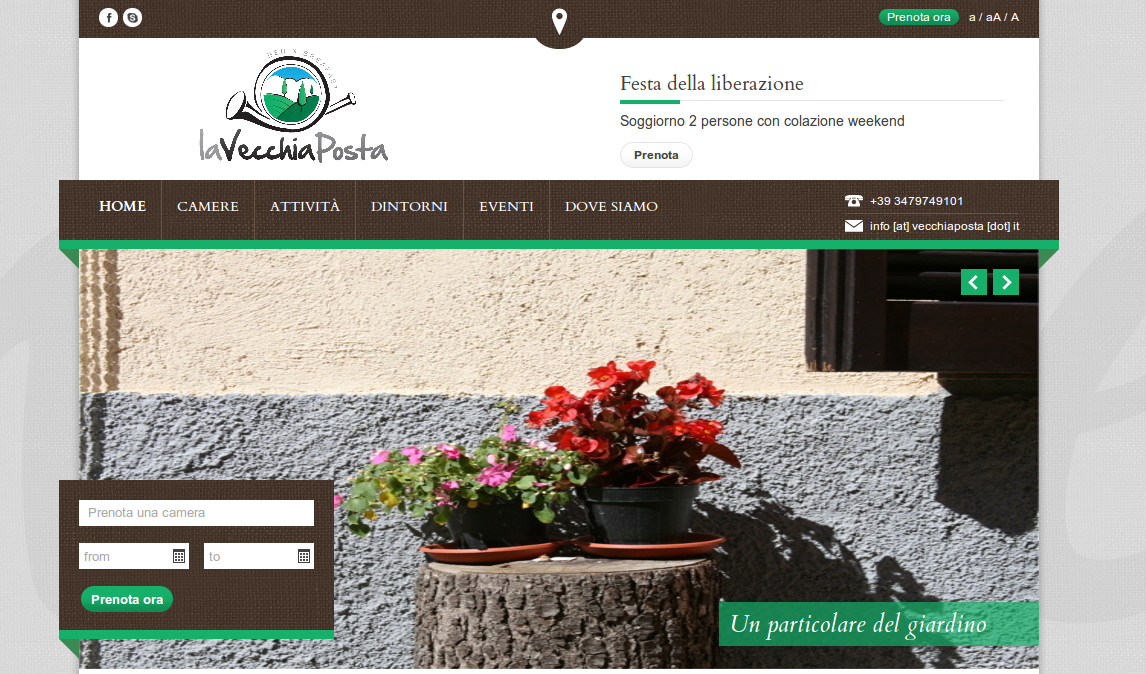
\includegraphics[width=0.9\textwidth,keepaspectratio=true]{../img/layoutHome}
    \centering
    \caption{Layout colori: header e slider}%
    \label{fig:header_slider}%
\end{figure}

La scelta dei colori del layout è stata fatta sulla base dei colori del logo dell'azienda.
Lo sfondo del tema è di un grigio {\color[RGB]{220, 220, 220} grigio del logo} DCDCDC.
Per i colori dominanti del tema sono stati scelti il marrone ed il verde, rispettando le ipotesi del documento dei requisiti in allegato.

Il colore marrone è stato utilizzato come sfondo della barra di navigazione principale, per la social bar e per il footer.
{\color[RGB]{69, 53, 42} verde del logo} \#45352A
\begin{picture}(2,2)
\put(1,1){\color[RGB]{22, 176, 106} grigio del logo}
\end{picture}

\begin{picture}(2,2)
\put(0,0){\dashbox{0.2}(20,20)[s]{\color}}
\end{picture}

Il colo verde {\color[RGB]{22, 176, 106} grigio del logo} \#16B06A invece è stato utilizzato come bordo inferiore della barra di navigazione, per i controller dello slider, per il caption dell'immagini dello slider
e per il bottone prenota nella social bar. L'utilizzo del colore verde è stato utilizzato anche per enfatizzare gli elementi ``titolo sezione''.


\newpage
\subsection*{Dimensione componenti}


\section*{Tipografia}

\end{document}          